% Lab 1 "Cloud Computing": Blowfish encryption on PARCS-Python in AWS.
% Build:  cd report && latexmk -xelatex report.tex
%    or:  xelatex report.tex && xelatex report.tex
\documentclass[a4paper,12pt]{article}

\usepackage{fontspec}
\usepackage{polyglossia}
\setdefaultlanguage{ukrainian}
\setotherlanguage{english}
% CM Unicode fonts ship with TeX Live / Overleaf; loading by file name works everywhere.
\setmainfont{cmunrm.otf}[BoldFont=cmunbx.otf, ItalicFont=cmunti.otf, BoldItalicFont=cmunbi.otf]
\setsansfont{cmunss.otf}[BoldFont=cmunsx.otf, ItalicFont=cmunsi.otf, BoldItalicFont=cmunso.otf]
\setmonofont{cmuntt.otf}[BoldFont=cmuntb.otf, ItalicFont=cmunit.otf, BoldItalicFont=cmuntx.otf]

\usepackage[margin=2.2cm]{geometry}
\usepackage{amsmath,amssymb}
\usepackage{graphicx}
\usepackage{booktabs}
\usepackage{longtable}
\usepackage{caption}
\usepackage{float}
\usepackage{xcolor}
\usepackage{listings}
\usepackage{tikz}
\usetikzlibrary{arrows.meta,positioning,calc,fit,shapes.geometric}
\usepackage{algorithm}
\usepackage{algpseudocode}
\usepackage{enumitem}
\usepackage[hidelinks]{hyperref}

\graphicspath{{figures/}{screenshots/}}
\setlist{itemsep=2pt,topsep=4pt}
\emergencystretch=3em
\captionsetup{font=small,labelfont=bf}
\floatname{algorithm}{Алгоритм}
\renewcommand{\listalgorithmname}{Список алгоритмів}
\algrenewcommand\algorithmicrequire{\textbf{Вхід:}}
\algrenewcommand\algorithmicensure{\textbf{Вихід:}}

\definecolor{codebg}{HTML}{F6F6F4}
\definecolor{codekw}{HTML}{1F5FA8}
\definecolor{codecm}{HTML}{6A6A66}
\definecolor{codestr}{HTML}{A8521F}
\lstset{
  language=Python, basicstyle=\ttfamily\small, backgroundcolor=\color{codebg},
  keywordstyle=\color{codekw}\bfseries, commentstyle=\color{codecm}\itshape,
  stringstyle=\color{codestr}, frame=single, rulecolor=\color{black!15},
  framesep=4pt, xleftmargin=6pt, xrightmargin=6pt, breaklines=true,
  columns=fullflexible, keepspaces=true, showstringspaces=false,
  numbers=left, numberstyle=\tiny\color{codecm}, numbersep=6pt,
}
\renewcommand{\lstlistingname}{Лістинг}

% Placeholder for a screenshot that is not available yet.
\newcommand{\screenshotplaceholder}[1]{%
  \fbox{\parbox[c][4.5cm][c]{0.85\textwidth}{\centering\small\color{black!60}%
  Місце для скріншота:\\[2pt] #1}}}

\begin{document}

% =====================================================================
% Title page
% =====================================================================
\begin{titlepage}
  \centering
  {\large КИЇВСЬКИЙ НАЦІОНАЛЬНИЙ УНІВЕРСИТЕТ\\ імені ТАРАСА ШЕВЧЕНКА\par}
  \vspace{0.6cm}
  {\large Факультет комп'ютерних наук та кібернетики\par}
  \vspace{4cm}
  {\Large Дисципліна «Хмарні обчислення»\par}
  \vspace{0.8cm}
  {\LARGE\bfseries Лабораторна робота №1\par}
  \vspace{0.6cm}
  {\Large Паралельне шифрування алгоритмом Blowfish\\ на платформі PARCS-Python у хмарі AWS\par}
  \vfill
  \begin{flushright}
    \begin{tabular}{l}
      Виконала:\\
      студентка групи МІ-41\\
      Уточкіна Яна Максимівна
    \end{tabular}
  \end{flushright}
  \vspace{2.5cm}
  {\large Київ --- 2026\par}
\end{titlepage}

\tableofcontents
\newpage

% =====================================================================
\section{Мета і постановка задачі}
% =====================================================================
\textbf{Мета роботи:} набути практичних навичок розгортання системи паралельних
обчислень ПАРКС у хмарному середовищі, реалізувати послідовний і паралельний
варіанти обраного алгоритму та дослідити, як змінюється час виконання залежно від
кількості обчислювальних вузлів.

\textbf{Завдання} (згідно з методичними вказівками):
\begin{enumerate}
  \item Обрати задачу паралельного програмування і платформу ПАРКС для її реалізації.
  \item Розгорнути систему ПАРКС у хмарному середовищі.
  \item Протестувати послідовний і паралельний алгоритми в хмарі для різної кількості воркерів.
  \item Оформити звіт з описом алгоритмів і порівнянням результатів.
  \item Завантажити код проєкту на GitHub.
\end{enumerate}

\textbf{Обрані параметри роботи:}
\begin{itemize}
  \item задача --- шифрування даних блоковим шифром \textbf{Blowfish};
  \item платформа --- \textbf{PARCS-Python}~\cite{hummer-parcs};
  \item хмара --- \textbf{Amazon Web Services (AWS)}, безкоштовний план (Free plan)~\cite{aws-free-plan};
  \item конфігурації: послідовний алгоритм і паралельний з 1, 2, 3, 4 воркерами;
        обсяги даних 1, 4, 16 і 64~МБ, по 5 повторів кожного вимірювання.
\end{itemize}

Шифрування великих обсягів даних --- природна задача для паралелізму за даними
(data parallelism): за правильно обраного режиму роботи шифру різні частини
даних можна обробляти незалежно на різних вузлах і без обміну між ними.

% =====================================================================
\section{Алгоритм шифрування Blowfish}
% =====================================================================
\subsection{Історія та загальні характеристики}
Blowfish запропонував Брюс Шнайєр у 1993~році~\cite{schneier-blowfish} як швидку,
вільну від патентів альтернативу DES. Основні характеристики:
\begin{itemize}
  \item розмір блоку --- 64 біти (8 байтів);
  \item довжина ключа --- від 32 до 448 бітів (4--56 байтів);
  \item 16 раундів мережі Фейстеля;
  \item ключезалежні S-блоки: чотири таблиці по 256 32-бітних слів;
  \item P-масив з 18 32-бітних підключів.
\end{itemize}
Сьогодні Blowfish вважається застарілим через малий розмір блоку (64 біти робить
його вразливим до атак на основі парадоксу днів народження при шифруванні
гігабайтів даних одним ключем), і для нових систем рекомендовано AES. Утім,
завдяки простій і наочній структурі він добре підходить для навчальної реалізації.

\subsection{Мережа Фейстеля}
Блок ділиться на дві 32-бітні половини $L$ і $R$. У кожному з 16 раундів
\[
  L \leftarrow L \oplus P_i,\qquad R \leftarrow R \oplus F(L),\qquad (L, R) \leftarrow (R, L),
  \qquad i = 0,\dots,15.
\]
Після 16 раундів останній обмін половин скасовується, і виконується вихідне
«відбілювання»: $R \leftarrow R \oplus P_{16}$, $L \leftarrow L \oplus P_{17}$.
Схему подано на рис.~\ref{fig:feistel}.

\begin{figure}[H]
  \centering
  \begin{tikzpicture}[
      font=\small, >=Stealth,
      box/.style={draw, minimum width=1.6cm, minimum height=0.7cm},
      xorn/.style={draw, circle, inner sep=0pt, minimum size=0.42cm,
                   path picture={\draw (path picture bounding box.north) -- (path picture bounding box.south)
                                       (path picture bounding box.west) -- (path picture bounding box.east);}},
      fbox/.style={draw, fill=black!6, minimum width=1.0cm, minimum height=0.7cm}]
    \node[box] (L0) at (0,0) {$L$ (32)};
    \node[box] (R0) at (5,0) {$R$ (32)};
    \node[xorn] (x1) at (0,-1.2) {};
    \node[left=0.3cm of x1] (p0) {$P_i$};
    \node[fbox] (F) at (2.5,-2.2) {$F$};
    \node[xorn] (x2) at (5,-2.2) {};
    \draw[->] (L0) -- (x1);
    \draw[->] (p0) -- (x1);
    \draw[->] (x1) -- (0,-2.2) -- (F);
    \draw[->] (F) -- (x2);
    \draw[->] (R0) -- (x2);
    \draw[->] (0,-2.2) -- (0,-2.9) -- (5,-3.9) -- (5,-4.4);
    \draw[->] (x2) -- (5,-2.9) -- (0,-3.9) -- (0,-4.4);
    \node[box, below=0cm of {(0,-4.4)}, anchor=north] {нове $L$};
    \node[box, below=0cm of {(5,-4.4)}, anchor=north] {нове $R$};
    \node[align=left, anchor=west] at (6.4,-2.2) {повторюється\\ 16 разів,\\ $i = 0..15$};
  \end{tikzpicture}
  \caption{Один раунд мережі Фейстеля в Blowfish}
  \label{fig:feistel}
\end{figure}

Розшифрування виконує ту саму мережу, але підключі $P_{17}, P_{16}, \dots, P_0$
застосовуються у зворотному порядку. Тому функцію $F$ не потрібно обертати.

\subsection{Функція F}
32-бітне слово $x$ розбивається на чотири байти $a, b, c, d$ (від старшого до
молодшого), і кожен байт є індексом в одній із чотирьох S-таблиць:
\[
  F(x) = \Bigl(\bigl(S_0[a] + S_1[b]\bigr) \oplus S_2[c]\Bigr) + S_3[d] \pmod{2^{32}}.
\]
Чергування додавання за модулем $2^{32}$ і XOR робить функцію нелінійною, а
залежність S-таблиць від ключа ускладнює диференціальний і лінійний криптоаналіз.

\subsection{Розгортання ключа (key schedule)}
\begin{enumerate}
  \item P-масив і S-таблиці заповнюються шістнадцятковими цифрами дробової частини
        числа~$\pi$: $18 + 4\cdot256 = 1042$ слова, тобто 8336 hex-цифр.
        У цій роботі їх обчислено програмно за формулою Мечіна
        $\pi = 16\arctan\frac{1}{5} - 4\arctan\frac{1}{239}$
        у цілочисельній арифметиці (скрипт \texttt{gen\_pi\_constants.py}),
        а не скопійовано з готових таблиць.
  \item Ключ циклічно накладається операцією XOR на P-масив: $P_0 \oplus=$ байти ключа 0--3,
        $P_1 \oplus=$ байти 4--7 і т.\,д. (короткий ключ повторюється).
  \item Нульовий блок шифрується поточними таблицями; результат замінює $P_0, P_1$.
        Результат шифрується знову і замінює $P_2, P_3$, і так далі для всього P-масиву
        та всіх S-таблиць. Усього виконується $(18 + 1024)/2 = 521$ шифрування.
\end{enumerate}
Через це створення об'єкта шифру з новим ключем порівняно дороге, зате шифрування
окремого блоку --- дешеве.

\subsection{Режими роботи та придатність до розпаралелювання}
Блоковий шифр перетворює лише 8 байтів, тому для довших повідомлень потрібен режим
роботи~\cite{nist-sp800-38a}. Реалізовано три режими:
\begin{itemize}
  \item \textbf{ECB} (Electronic Codebook): $C_i = E_K(P_i)$. Блоки незалежні, отже
        розпаралелюються, але однакові блоки відкритого тексту дають однакові
        блоки шифротексту, що розкриває структуру даних. Потрібне доповнення до
        кратності 8 байтам: використано \textbf{PKCS\#7} (додається $N$ байтів зі значенням $N$, $1 \le N \le 8$).
  \item \textbf{CBC} (Cipher Block Chaining): $C_i = E_K(P_i \oplus C_{i-1})$, $C_{-1} = IV$.
        \emph{Шифрування не розпаралелюється}: щоб почати блок $i$, потрібен уже
        обчислений $C_{i-1}$, тобто існує ланцюгова залежність через усе повідомлення.
        Розшифрування $P_i = D_K(C_i) \oplus C_{i-1}$ розпаралелюється, бо всі $C_i$ відомі наперед.
  \item \textbf{CTR} (Counter): $C_i = P_i \oplus E_K(\mathit{nonce} \,\|\, (c_0 + i))$.
        Блоки повністю незалежні: будь-який фрагмент, що починається з байта
        $\mathit{off}$ (кратного 8), можна обробити окремо, якщо задати початковий
        лічильник $c_0 = \mathit{off}/8$. Доповнення не потрібне, а шифрування і
        розшифрування --- одна й та сама операція.
\end{itemize}
\textbf{Для паралельної версії обрано режим CTR}: він безпечніший за ECB і, на
відміну від CBC, дозволяє шифрувати частини даних незалежно. Формат лічильникового
блоку: 4 байти nonce і 32-бітний лічильник у порядку big-endian. Це збігається з
\texttt{Blowfish.new(key, MODE\_CTR, nonce=..., initial\_value=...)} бібліотеки
pycryptodome~\cite{pycryptodome}, що дозволило звірити результати.

\subsection{Реалізація}
Blowfish реалізовано з нуля на чистому Python (\texttt{src/blowfish.py}), без
сторонніх криптобібліотек. Код сумісний з Python~3 і Python~2.7, оскільки
вузли PARCS-Python працюють саме на Python~2.7. Для швидкодії в циклі виконується
по два раунди за ітерацію (без явного обміну половин), а функцію $F$ вбудовано
в цикл (лістинг~\ref{lst:encrypt}). Дані перетворюються на списки 32-бітних слів
через \texttt{struct.unpack} сегментами по 64~КіБ, щоб обмежити використання пам'яті.

\begin{lstlisting}[caption={Шифрування одного блоку (два раунди Фейстеля за ітерацію)},label={lst:encrypt}]
def encrypt_words(self, left, right):
    P = self.P
    S0, S1, S2, S3 = self.S
    for i in xrange(0, ROUNDS, 2):
        left ^= P[i]
        right ^= ((((S0[left >> 24] + S1[(left >> 16) & 0xFF]) & MASK32)
                   ^ S2[(left >> 8) & 0xFF]) + S3[left & 0xFF]) & MASK32
        right ^= P[i + 1]
        left ^= ((((S0[right >> 24] + S1[(right >> 16) & 0xFF]) & MASK32)
                  ^ S2[(right >> 8) & 0xFF]) + S3[right & 0xFF]) & MASK32
    # undo the last swap and apply output whitening with P[16], P[17]
    return right ^ P[ROUNDS + 1], left ^ P[ROUNDS]
\end{lstlisting}

\subsection{Перевірка коректності}
Набір тестів \texttt{pytest} (192 тести, усі проходять) перевіряє:
\begin{itemize}
  \item 34 офіційні ECB-вектори Е.~Янга, опубліковані на сайті Шнайєра~\cite{schneier-vectors};
  \item 24 вектори зі змінною довжиною ключа (1--24 байти) і CBC-вектор з того ж файлу;
  \item збіг з pycryptodome у режимах ECB, CBC, CTR для ключів 4--56 байтів, різних довжин даних
        (зокрема некратних 8) і різних початкових лічильників;
  \item roundtrip: $D(E(m)) = m$ для всіх режимів, коректність і відхилення некоректного PKCS\#7;
  \item рівномірність і вирівнювання розбиття даних та рівність
        «паралельний CTR = послідовний CTR» для 1--5 частин;
  \item наскрізний запуск PARCS-розв'язувача з імітацією воркерів.
\end{itemize}
Додатково розв'язувач перевірено на справжньому кластері PARCS у локальному Docker
(Python~2.7.13): SHA-256 шифротексту збігся з результатом Python~3.

% =====================================================================
\section{Платформа ПАРКС і хмарне середовище AWS}
% =====================================================================
\subsection{Технологія ПАРКС}
ПАРКС (PARCS --- PARallel Computer System) --- технологія паралельного
програмування, розроблена на факультеті комп'ютерних наук та кібернетики КНУ
імені Тараса Шевченка. Відома реалізація PARCS-JAVA~\cite{parcs-java}, а також
реалізації для інших мов, зокрема Python~\cite{parcs-overview}. Програма в ПАРКС
складається з керуючого модуля і модулів, які виконуються на вузлах обчислювальної
мережі й обмінюються даними через канали.

\subsection{PARCS-Python}
Використано реалізацію PARCS-Python~\cite{hummer-parcs} (Docker-образ
\texttt{hummer12007/parcs-node}, Python~2.7). Її архітектура:
\begin{itemize}
  \item \textbf{master} --- Flask-сервер з веб-інтерфейсом (порт 8080): реєструє воркерів,
        приймає завдання (файл розв'язку \texttt{solution.py} і вхідний файл), ставить їх у
        чергу і запускає \texttt{Solver.solve()};
  \item \textbf{worker} --- той самий образ, запущений з параметром \texttt{worker <IP master>};
        при старті реєструється на master, а для кожного завдання піднімає
        Pyro4-демон~\cite{pyro4} з об'єктом класу \texttt{Solver};
  \item \textbf{розв'язок} --- один Python-файл з класом \texttt{Solver}. На master
        конструктор отримує список Pyro4-проксі воркерів, а методи з декоратором
        \texttt{@expose} викликаються віддалено (RPC);
  \item вузли спілкуються на випадкових TCP-портах (Flask воркера і Pyro4),
        тому контейнери запускаються з \texttt{--network host}.
\end{itemize}
Оскільки PARCS передає на вузли лише один файл, реалізацію Blowfish вбудовано в
розв'язок під час збирання (\texttt{scripts/build\_solver.py} $\to$ \texttt{build/solver.py}).

\subsection{AWS: умови безкоштовного плану}
Для акаунтів, створених після 15.07.2025, AWS надає 100~доларів кредитів (і до
100~доларів додатково за виконання завдань) на 6 місяців. На Free plan гроші з
картки не списуються: після вичерпання кредитів або завершення строку акаунт
закривається~\cite{aws-free-plan}. Free-tier-типи EC2 для таких акаунтів:
\texttt{t3.micro}, \texttt{t3.small}, \texttt{t4g.micro}, \texttt{t4g.small},
\texttt{c7i-flex.large}, \texttt{m7i-flex.large}~\cite{aws-ec2-free}.

За замовчуванням квота «Running On-Demand Standard instances» становила 5~vCPU, тобто
лише дві VM по 2~vCPU. Через Service Quotas її збільшено до 16~vCPU.

% =====================================================================
\section{Послідовний алгоритм}
% =====================================================================
Послідовний алгоритм шифрує весь масив даних в одному процесі (алгоритм~\ref{alg:seq}).
У хмарі його виконує master-вузол у тому самому середовищі (Docker-образ PARCS,
Python~2.7), що й воркери. Вимірюваний час включає розгортання ключа і
шифрування, але не читання файлу.

\begin{algorithm}[H]
  \caption{Послідовне шифрування Blowfish-CTR}\label{alg:seq}
  \begin{algorithmic}[1]
    \Require ключ $K$, nonce $N$ (4 байти), дані $M$ довжиною $n$ байтів
    \Ensure шифротекст $C$, $|C| = n$
    \State $\mathit{cipher} \gets \textsc{KeySchedule}(K)$ \Comment{521 шифрування}
    \For{$i \gets 0$ \textbf{to} $\lceil n/8 \rceil - 1$}
      \State $k_i \gets \mathit{cipher}.\textsc{Encrypt}(N \,\|\, i)$ \Comment{ключовий потік}
      \State $C[8i \,..\, 8i+7] \gets M[8i \,..\, 8i+7] \oplus k_i$ \Comment{останній блок може бути неповним}
    \EndFor
    \State \Return $C$
  \end{algorithmic}
\end{algorithm}

Складність --- $\Theta(n)$ операцій шифрування блоку (по 16 раундів).
Окрема утиліта \texttt{src/sequential.py} дозволяє шифрувати й розшифровувати
довільні файли з командного рядка.

% =====================================================================
\section{Паралельний алгоритм}
% =====================================================================
\subsection{Схема розподілу даних}
Master розбиває дані на $p$ неперервних частин, вирівняних на межу 8-байтового блоку,
і надсилає кожному воркеру його частину разом із ключем, nonce і початковим
значенням лічильника (рис.~\ref{fig:scheme}, алгоритм~\ref{alg:par}).

\begin{figure}[H]
  \centering
  \begin{tikzpicture}[font=\small, >=Stealth,
      node distance=0.5cm,
      blk/.style={draw, minimum height=0.65cm, fill=#1},
      wk/.style={draw, rounded corners=2pt, minimum width=2.6cm, minimum height=0.9cm, align=center, fill=black!4}]
    % plaintext
    \node[anchor=west] at (-0.2,1.0) {Відкритий текст $M$ ($n$ байтів):};
    \node[blk=blue!12, minimum width=3cm, anchor=west] (m1) at (0,0.3) {$[s_1, e_1)$};
    \node[blk=orange!15, minimum width=3cm, right=0cm of m1] (m2) {$[s_2, e_2)$};
    \node[blk=green!12, minimum width=3cm, right=0cm of m2] (m3) {$\dots$};
    \node[blk=yellow!20, minimum width=3cm, right=0cm of m3] (m4) {$[s_p, n)$};
    % master
    \node[draw, thick, rounded corners=3pt, minimum width=12cm, minimum height=0.9cm, align=center, fill=black!8]
      (master) at (6,-1.3) {\textbf{master}: розбиття, base64, розсилка; збирання результатів у порядку частин};
    % workers
    \node[wk] (w1) at (1.5,-3.4) {воркер 1\\ $c_0 = s_1/8$};
    \node[wk] (w2) at (4.5,-3.4) {воркер 2\\ $c_0 = s_2/8$};
    \node[wk] (w3) at (7.5,-3.4) {\dots};
    \node[wk] (w4) at (10.5,-3.4) {воркер $p$\\ $c_0 = s_p/8$};
    \foreach \w in {w1,w2,w4} {
      \draw[->] ([xshift=-4mm]master.south -| \w) -- ([xshift=-4mm]\w.north);
      \draw[<-] ([xshift=4mm]master.south -| \w) -- ([xshift=4mm]\w.north);
    }
    \node[font=\scriptsize, align=left] at (3.0,-2.35) {$\downarrow$ частина, $K$, $N$, $c_0$ \quad $\uparrow$ шифротекст, $t_{\text{обч}}$};
    % ciphertext
    \node[blk=blue!12, minimum width=3cm, anchor=west] (c1) at (0,-5.0) {$C[s_1, e_1)$};
    \node[blk=orange!15, minimum width=3cm, right=0cm of c1] (c2) {$C[s_2, e_2)$};
    \node[blk=green!12, minimum width=3cm, right=0cm of c2] (c3) {$\dots$};
    \node[blk=yellow!20, minimum width=3cm, right=0cm of c3] (c4) {$C[s_p, n)$};
    \node[anchor=west] at (-0.2,-5.7) {Шифротекст $C$ = конкатенація частин (байт-у-байт як у послідовному алгоритмі)};
  \end{tikzpicture}
  \caption{Схема розподілу даних master $\to$ workers}
  \label{fig:scheme}
\end{figure}

\begin{algorithm}[H]
  \caption{Паралельне шифрування Blowfish-CTR на PARCS (master)}\label{alg:par}
  \begin{algorithmic}[1]
    \Require ключ $K$, nonce $N$, дані $M$ ($n$ байтів), воркери $w_1..w_p$
    \Ensure шифротекст $C$
    \State $B \gets \lceil n/8 \rceil$; \quad $q, r \gets \lfloor B/p \rfloor,\ B \bmod p$
    \For{$j \gets 1$ \textbf{to} $p$} \Comment{частина $j$: $q$ або $q+1$ блоків}
      \State $s_j \gets 8 \cdot \bigl((j-1) q + \min(j-1, r)\bigr)$; \quad $e_j \gets \min\bigl(s_j + 8(q + [j \le r]),\ n\bigr)$
    \EndFor
    \ForAll{$j \in 1..p$ \textbf{паралельно}} \Comment{окремий потік на кожного воркера}
      \State $R_j \gets w_j.\textsc{EncryptChunk}\bigl(K, N, c_0 = s_j/8, \textsc{Base64}(M[s_j, e_j))\bigr)$
    \EndFor
    \State \Return $C \gets \textsc{Base64Decode}(R_1) \,\|\, \dots \,\|\, \textsc{Base64Decode}(R_p)$
  \end{algorithmic}
\end{algorithm}

На воркері метод \texttt{encrypt\_chunk} декодує дані, шифрує їх у режимі CTR з
лічильником $c_0$ і повертає шифротекст разом із виміряним часом чистих обчислень:

\begin{lstlisting}[caption={Метод воркера, що викликається через Pyro4}]
@staticmethod
@expose
def encrypt_chunk(key_hex, nonce_hex, initial_counter, data_b64):
    t0 = time.time()
    chunk = base64.b64decode(data_b64)
    t1 = time.time()
    cipher = Blowfish(binascii.unhexlify(str(key_hex)))
    encrypted = cipher.ctr_xcrypt(chunk, binascii.unhexlify(str(nonce_hex)),
                                  int(initial_counter))
    t2 = time.time()
    encoded = _b64encode(encrypted)
    t3 = time.time()
    return [encoded, t2 - t1, (t1 - t0) + (t3 - t2)]
\end{lstlisting}

Дані передаються в base64, бо серіалізатор Pyro4 під Python~2 надійно передає
текстові рядки, а довільні бінарні --- ні. Master викликає воркерів з окремих
потоків, тому розв'язок працює незалежно від того, чи надає PARCS синхронні,
чи асинхронні проксі. Перед вимірюваннями виконується невимірюваний «прогрів»
усіх воркерів, щоб відкрити з'єднання.

\subsection{Обґрунтування коректності}
\begin{enumerate}
  \item Межі частин $s_j$ кратні 8, частини не перетинаються і разом покривають
        $[0, n)$: $s_1 = 0$, $s_{j+1} = e_j$, $e_p = n$.
  \item У режимі CTR блок з номером $i$ (байти $8i..8i+7$) шифрується як
        $M_i \oplus E_K(N \,\|\, i)$ і залежить лише від $K$, $N$, $i$ та $M_i$.
  \item Воркер $j$ обробляє блоки з номерами $s_j/8, s_j/8 + 1, \dots$ і починає
        лічильник саме з $c_0 = s_j/8$, тобто кожен блок отримує той самий
        лічильник, що й у послідовному алгоритмі.
  \item Неповний останній блок може бути лише в останній частині, і обробляється
        так само, як у послідовному алгоритмі (використовується префікс ключового потоку).
  \item Master склеює результати в порядку частин, отже $C_{\text{пар}} = C_{\text{посл}}$
        байт-у-байт.
\end{enumerate}
Це твердження перевірялося в кожному прогоні: розв'язувач порівнює SHA-256
шифротексту з результатом послідовного алгоритму. Усі 100 вимірювальних прогонів
пройшли цю перевірку.

\subsection{Що вимірюється}
Для кожного прогону фіксуються:
\begin{itemize}
  \item $T$ --- загальний час на master від початку розбиття до готового шифротексту;
  \item $T_{\text{обч}}$ --- час чистого шифрування на найповільнішому воркері;
  \item накладні витрати $T - T_{\text{обч}}$. Вони складаються з розбиття та base64 на master,
        передачі й серіалізації Pyro4 разом із base64 на воркерах, а також декодування й склеювання на master.
\end{itemize}

% =====================================================================
\section{Розгортання в хмарі AWS}
% =====================================================================
\subsection{Архітектура}
Кластер розгорнуто в регіоні \textbf{eu-north-1} (Стокгольм), зона доступності
eu-north-1b, у VPC за замовчуванням (рис.~\ref{fig:aws}).

\begin{figure}[H]
  \centering
  \begin{tikzpicture}[font=\small, >=Stealth,
      vm/.style={draw, rounded corners=2pt, fill=black!4, minimum width=2.5cm, minimum height=1.2cm, align=center}]
    \node[vm, fill=blue!8] (m) at (0,0) {\textbf{parcs-master}\\ c7i-flex.large\\ PARCS master :8080};
    \node[vm] (w1) at (-4.8,-2.8) {parcs-worker\\ c7i-flex.large};
    \node[vm] (w2) at (-1.6,-2.8) {parcs-worker\\ c7i-flex.large};
    \node[vm] (w3) at (1.6,-2.8) {parcs-worker\\ c7i-flex.large};
    \node[vm] (w4) at (4.8,-2.8) {parcs-worker\\ c7i-flex.large};
    \foreach \w in {w1,w2,w3,w4} \draw[<->] (m.south) -- (\w.north);
    \node[draw, dashed, rounded corners=4pt, inner sep=10pt, fit=(m)(w1)(w4),
          label={[anchor=north, font=\scriptsize]south:security group \texttt{parcs-sg}: між вузлами групи дозволено всі з'єднання}] (sg) {};
    \coordinate (sglabel) at ($(sg.south)+(0,-0.5)$);
    \node[draw, rounded corners=4pt, inner sep=6pt, fit=(sg)(sglabel),
          label={[anchor=south west, font=\scriptsize]north west:VPC за замовчуванням, eu-north-1}] {};
    \node[align=center] (me) at (0,2.6) {ноутбук студента};
    \draw[->] (me) -- node[right, font=\scriptsize] {SSH :22, HTTP :8080 --- лише з однієї IP} (m.north);
  \end{tikzpicture}
  \caption{Архітектура розгортання в AWS}
  \label{fig:aws}
\end{figure}

\begin{table}[H]
  \centering
  \caption{Параметри обчислювальних вузлів (дані зібрано скриптом \texttt{deploy/collect\_env.sh})}
  \begin{tabular}{ll}
    \toprule
    Кількість VM & 5: 1 master + 4 воркери \\
    Тип інстансу & \texttt{c7i-flex.large} (free-tier eligible) \\
    vCPU / пам'ять & 2 vCPU (1 ядро, 2 потоки) / 3.7 ГіБ \\
    Процесор & Intel Xeon Platinum 8488C \\
    ОС & Ubuntu 26.04.1 LTS \\
    Docker & 29.1.3 \\
    Образ PARCS & \texttt{hummer12007/parcs-node}, Python 2.7.13 \\
    Затримка master $\to$ воркер (ping) & 0.29--0.61 мс \\
    \bottomrule
  \end{tabular}
\end{table}

\subsection{Кроки розгортання}
Детальна інструкція наведена у файлі \texttt{deploy/AWS\_SETUP.md} репозиторію. Основні кроки:
\begin{enumerate}
  \item Збільшити квоту vCPU через Service Quotas (5 $\to$ 16).
  \item Створити пару ключів SSH (ED25519). Приватний ключ зберігається лише локально і не потрапляє в репозиторій.
  \item Створити security group \texttt{parcs-sg}: вхідні SSH (22) і HTTP (8080) лише з IP
        студента, а також усі з'єднання між членами самої групи (вузли PARCS використовують випадкові порти).
  \item Створити master-VM з \emph{User data} \texttt{deploy/user-data-master.sh}: скрипт
        встановлює Docker і запускає контейнер
        \texttt{docker run --network host -e PARCS\_ARGS=master hummer12007/parcs-node}.
  \item Створити 4 воркер-VM з \emph{User data} \texttt{deploy/user-data-worker.sh},
        передавши приватну IP master'а (\texttt{PARCS\_ARGS="worker <IP>"}).
  \item Перевірити реєстрацію воркерів у веб-інтерфейсі (рис.~\ref{fig:workers}).
  \item Скопіювати код на master, зібрати \texttt{solver.py}, згенерувати дані і запустити
        серію експериментів скриптом \texttt{run\_experiments.py}, який працює через HTTP API master'а.
  \item Після експериментів видалити всі ресурси: інстанси, диски, security group, ключі.
\end{enumerate}

\begin{figure}[H]
  \centering
  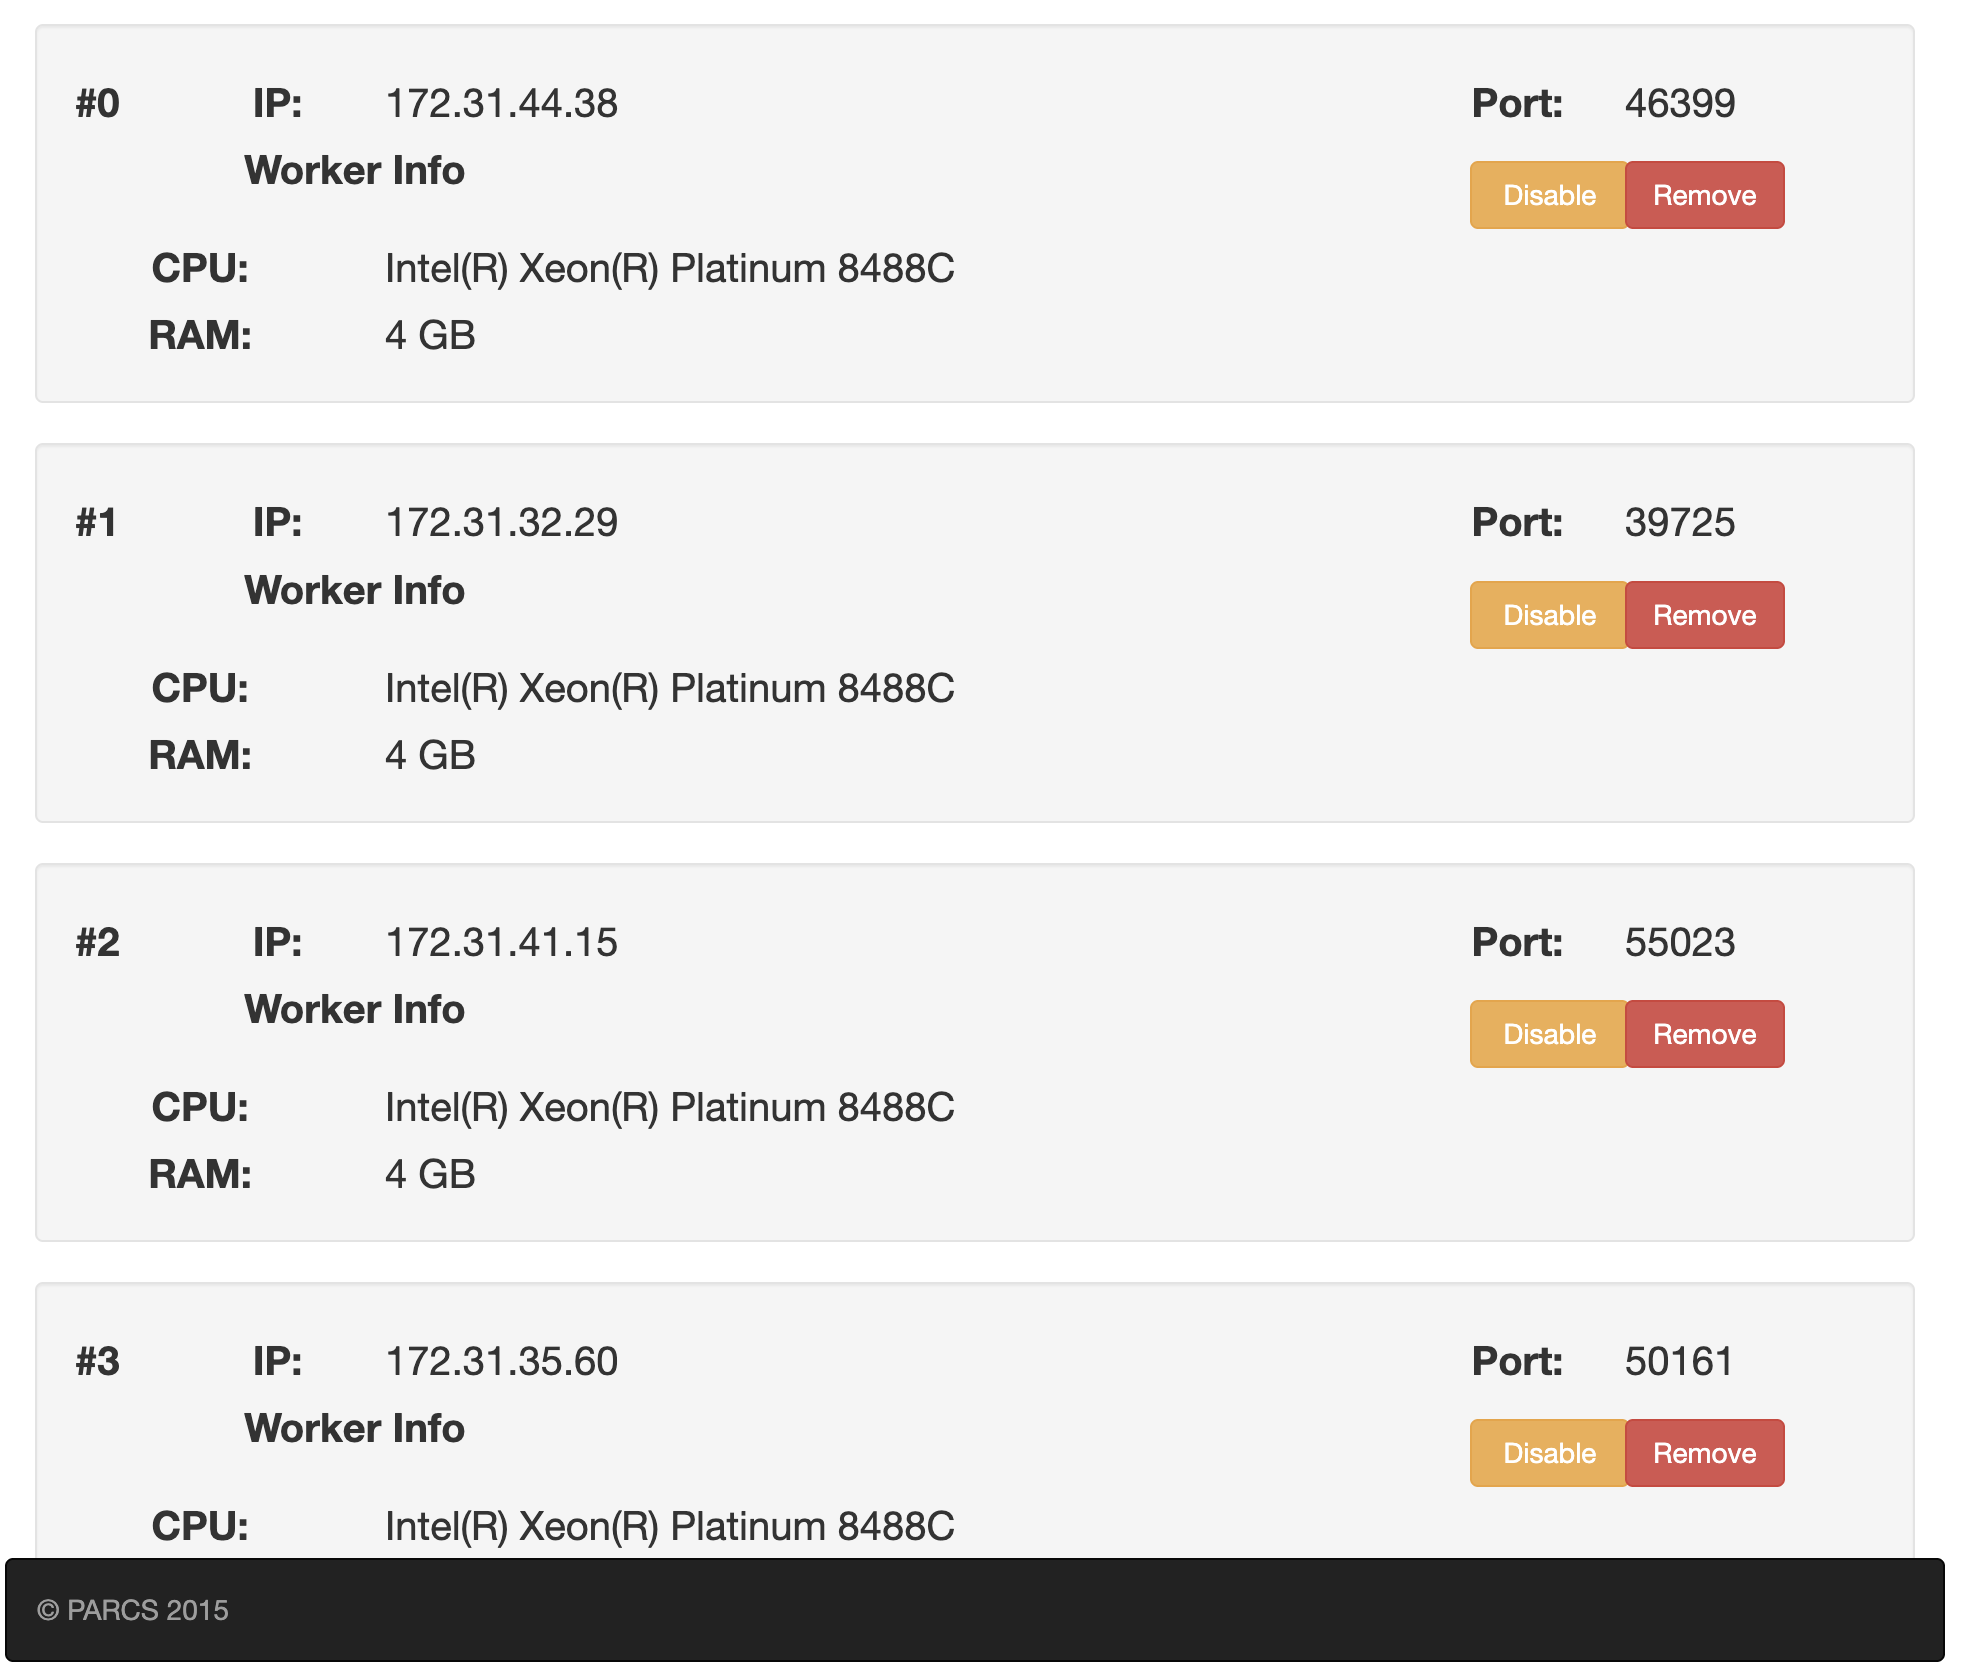
\includegraphics[width=0.85\textwidth]{parcs_workers.png}
  \caption{Веб-інтерфейс PARCS: зареєстровані воркери (приватні IP у VPC)}
  \label{fig:workers}
\end{figure}

\begin{figure}[H]
  \centering
  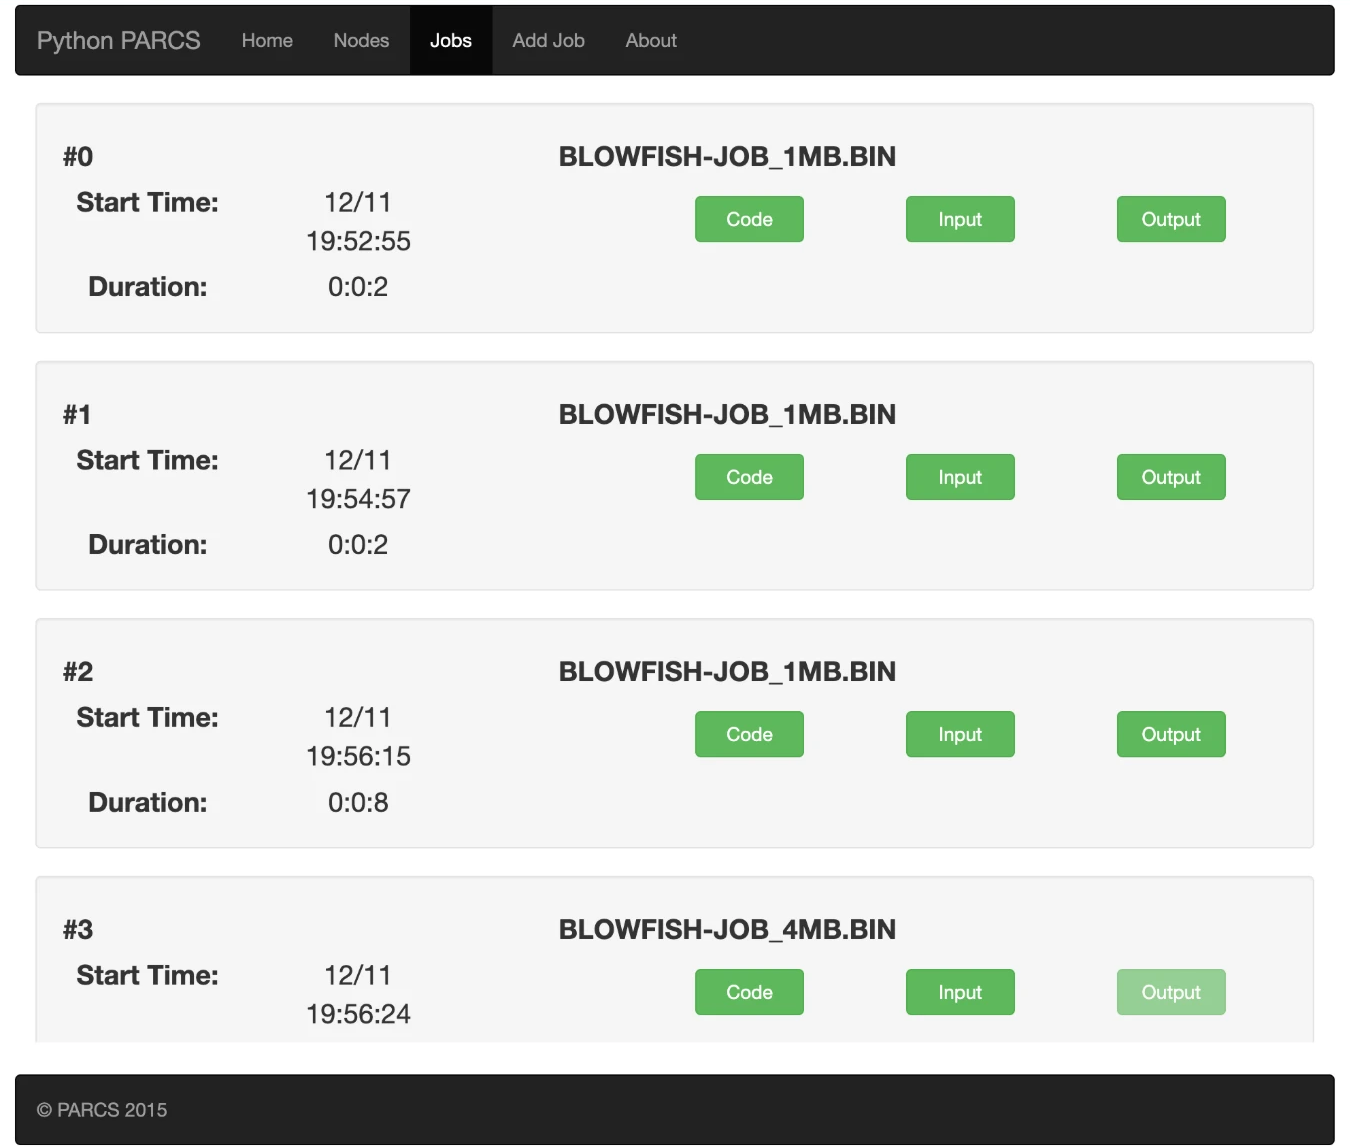
\includegraphics[width=0.75\textwidth]{parcs_jobs.png}
  \caption{Веб-інтерфейс PARCS: черга завдань під час серії експериментів}
  \label{fig:jobs}
\end{figure}

% Optional: add more screenshots (EC2 instance list, security group rules) here, e.g.
% \begin{figure}[H]\centering\includegraphics[width=0.85\textwidth]{ec2_instances.png}
% \caption{Запущені інстанси EC2}\end{figure}

% =====================================================================
\section{Експерименти}
% =====================================================================
\subsection{Методика}
\begin{itemize}
  \item Вхідні дані --- псевдовипадкові байти обсягом 1, 4, 16 і 64~МіБ
        (генератор \texttt{gen\_data.py}, фіксоване зерно), ключ 18 байтів, фіксований nonce.
  \item Для кожного обсягу одне завдання PARCS виконує послідовний алгоритм і паралельний з
        $p = 1, 2, 3, 4$ воркерами, по 5 повторів кожної конфігурації. Завдання запускалися
        по черзі, тому кластер не був зайнятий іншою роботою.
  \item Час вимірюється функцією \texttt{time.time()} на master (загальний) і на воркерах (обчислення).
        Таблиці містять середнє значення і стандартне відхилення за 5 повторами.
  \item Прискорення $S(p) = T_{\text{посл}} / T(p)$, ефективність $E(p) = S(p)/p$.
  \item Дата проведення: 12.11.2026.
\end{itemize}

\subsection{Результати}
\begin{longtable}{rrrrrrr}
  \caption{Середній час виконання (5 повторів), накладні витрати, прискорення та ефективність}\label{tab:results}\\
  \toprule
  МіБ & $p$ & $T$, с & $T_{\text{обч}}$, с & Накл., с & $S(p)$ & $E(p)$ \\
  \midrule
  \endfirsthead
  \toprule
  МіБ & $p$ & $T$, с & $T_{\text{обч}}$, с & Накл., с & $S(p)$ & $E(p)$ \\
  \midrule
  \endhead
  1 & посл. & 0.429 $\pm$ 0.004 & 0.429 & 0.000 & 1.00 & -- \\
1 & 1 & 0.443 $\pm$ 0.003 & 0.383 & 0.061 & 0.97 & 0.97 \\
1 & 2 & 0.251 $\pm$ 0.005 & 0.213 & 0.037 & 1.71 & 0.86 \\
1 & 3 & 0.177 $\pm$ 0.002 & 0.143 & 0.033 & 2.43 & 0.81 \\
1 & 4 & 0.138 $\pm$ 0.001 & 0.110 & 0.028 & 3.11 & 0.78 \\
\midrule
4 & посл. & 1.719 $\pm$ 0.005 & 1.719 & 0.000 & 1.00 & -- \\
4 & 1 & 1.794 $\pm$ 0.018 & 1.537 & 0.257 & 0.96 & 0.96 \\
4 & 2 & 0.971 $\pm$ 0.010 & 0.816 & 0.155 & 1.77 & 0.88 \\
4 & 3 & 0.681 $\pm$ 0.004 & 0.561 & 0.120 & 2.53 & 0.84 \\
4 & 4 & 0.529 $\pm$ 0.012 & 0.426 & 0.103 & 3.25 & 0.81 \\
\midrule
16 & посл. & 6.846 $\pm$ 0.021 & 6.846 & 0.000 & 1.00 & -- \\
16 & 1 & 7.319 $\pm$ 0.031 & 6.225 & 1.094 & 0.94 & 0.94 \\
16 & 2 & 3.937 $\pm$ 0.022 & 3.241 & 0.696 & 1.74 & 0.87 \\
16 & 3 & 2.764 $\pm$ 0.024 & 2.248 & 0.516 & 2.48 & 0.83 \\
16 & 4 & 2.172 $\pm$ 0.047 & 1.702 & 0.470 & 3.15 & 0.79 \\
\midrule
64 & посл. & 27.669 $\pm$ 0.213 & 27.669 & 0.000 & 1.00 & -- \\
64 & 1 & 29.692 $\pm$ 0.092 & 24.958 & 4.733 & 0.93 & 0.93 \\
64 & 2 & 16.885 $\pm$ 0.249 & 13.876 & 3.009 & 1.64 & 0.82 \\
64 & 3 & 11.815 $\pm$ 0.092 & 9.296 & 2.519 & 2.34 & 0.78 \\
64 & 4 & 9.074 $\pm$ 0.036 & 6.887 & 2.186 & 3.05 & 0.76 \\
\bottomrule

\end{longtable}

\begin{figure}[H]
  \centering
  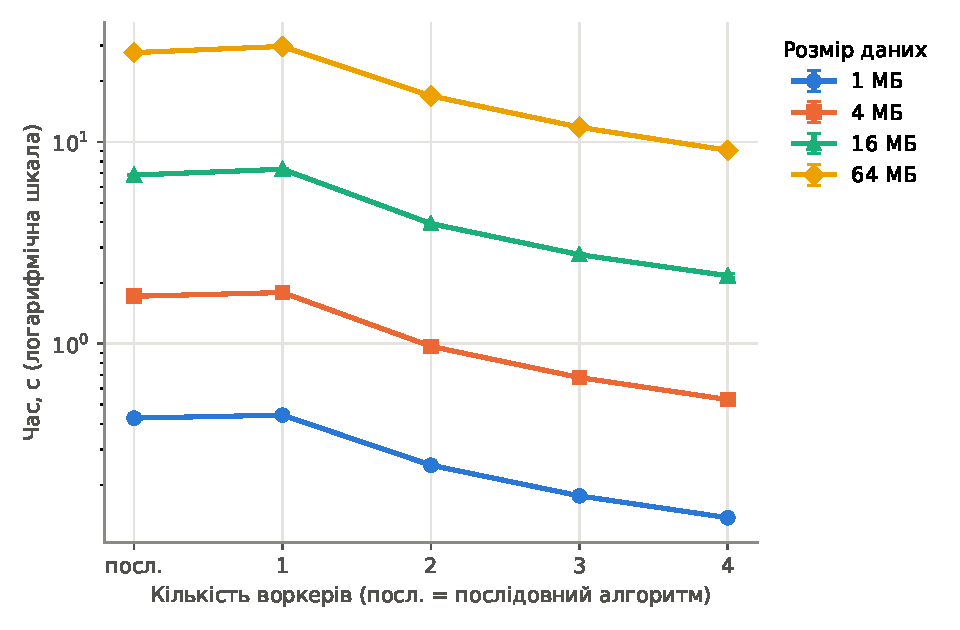
\includegraphics[width=0.8\textwidth]{time_vs_workers.pdf}
  \caption{Час виконання залежно від кількості воркерів (логарифмічна шкала; «посл.» --- послідовний алгоритм)}
  \label{fig:time}
\end{figure}

\begin{figure}[H]
  \centering
  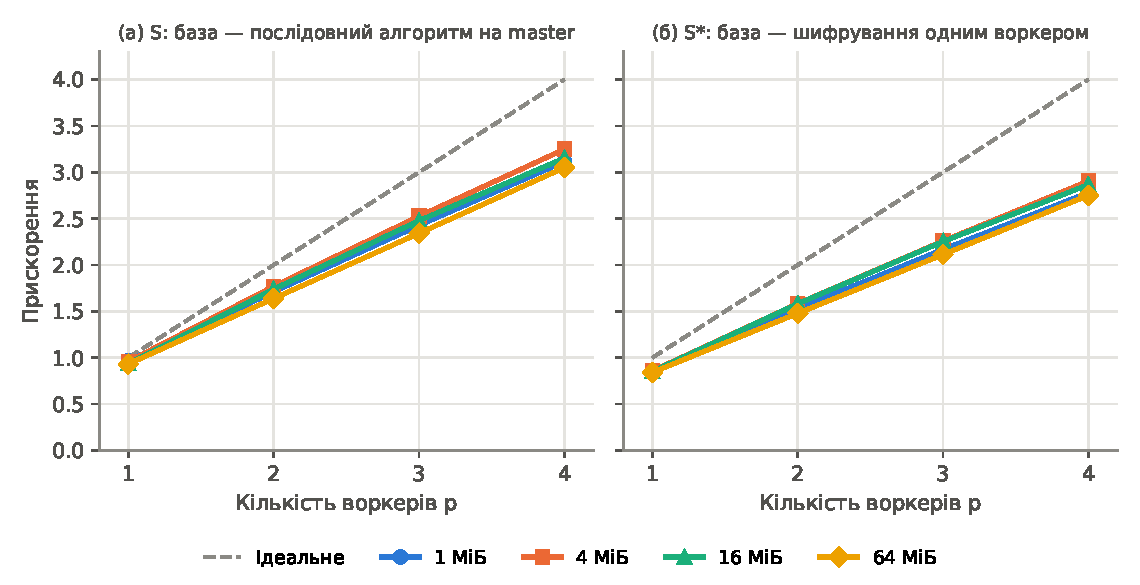
\includegraphics[width=0.8\textwidth]{speedup.pdf}
  \caption{Прискорення порівняно з ідеальним лінійним}
  \label{fig:speedup}
\end{figure}

\begin{figure}[H]
  \centering
  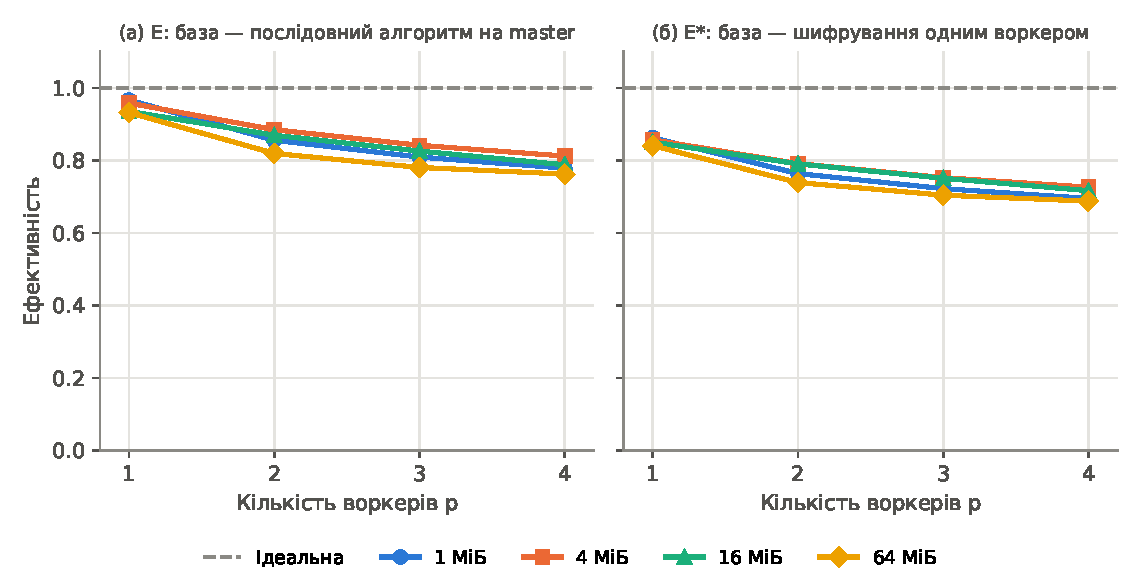
\includegraphics[width=0.8\textwidth]{efficiency.pdf}
  \caption{Ефективність паралельного алгоритму}
  \label{fig:efficiency}
\end{figure}

\begin{figure}[H]
  \centering
  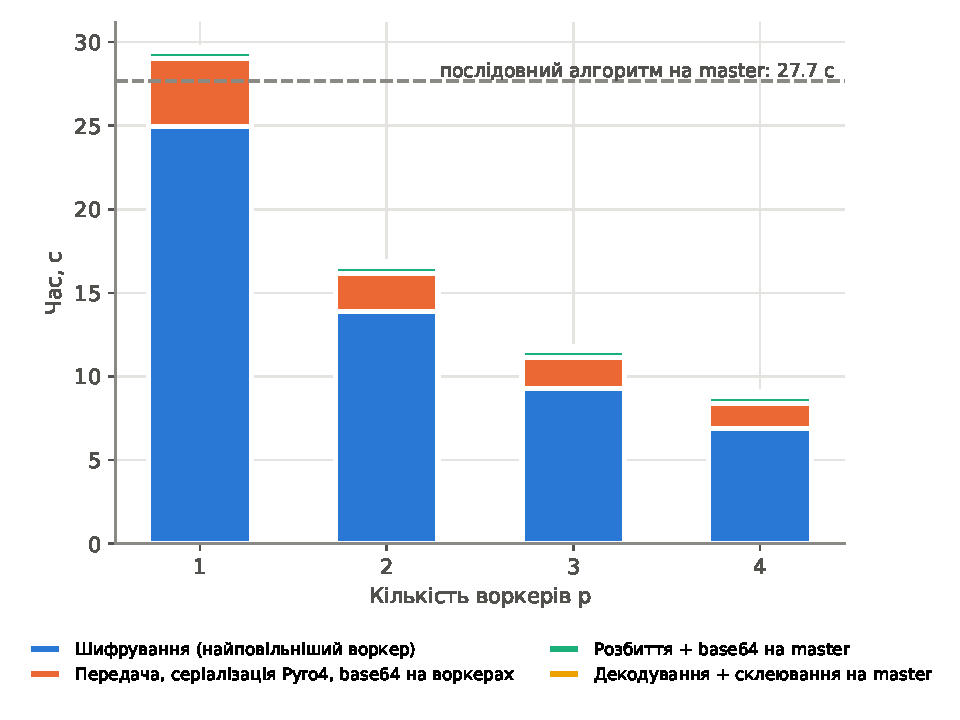
\includegraphics[width=0.8\textwidth]{breakdown_64mb.pdf}
  \caption{Складові часу виконання для 64~МіБ}
  \label{fig:breakdown}
\end{figure}

\begin{table}[H]
  \centering
  \caption{Емпірична послідовна частка Карпа--Флетта $e(p)$ і частка накладних витрат у загальному часі}
  \label{tab:kf}
  \begin{tabular}{r|rrr|rrrr}
    \toprule
    & \multicolumn{3}{c|}{$e(p) = \dfrac{1/S - 1/p}{1 - 1/p}$} & \multicolumn{4}{c}{$(T - T_{\text{обч}})/T$} \\
    МіБ & $p=2$ & $p=3$ & $p=4$ & $p=1$ & $p=2$ & $p=3$ & $p=4$ \\
    \midrule
    1 & 0.169 & 0.118 & 0.095 & 14\% & 15\% & 19\% & 20\% \\
4 & 0.130 & 0.094 & 0.077 & 14\% & 16\% & 18\% & 19\% \\
16 & 0.150 & 0.106 & 0.090 & 15\% & 18\% & 19\% & 22\% \\
64 & 0.221 & 0.141 & 0.104 & 16\% & 18\% & 21\% & 24\% \\
\bottomrule

  \end{tabular}
\end{table}

% =====================================================================
\section{Аналіз результатів і висновки}
% =====================================================================
\subsection{Аналіз}
\paragraph{Паралелізм дає суттєвий виграш.} На 4 воркерах прискорення становить
3.05--3.25 при ефективності 0.76--0.81 для всіх обсягів даних
(табл.~\ref{tab:results}, рис.~\ref{fig:speedup}). Причина в тому, що шифрування
в режимі CTR ділиться на повністю незалежні частини і воркерам не потрібно
обмінюватися даними між собою.

\paragraph{Один воркер повільніший за послідовний алгоритм.} $S(1) = 0.93$--$0.97$.
Обсяг обчислень той самий, але додаються кодування base64, серіалізація Pyro4,
передача даних мережею в обидва боки і склеювання. Ці накладні витрати становлять
14--16\,\% загального часу (табл.~\ref{tab:kf}).

\paragraph{Розмір даних майже не впливає на прискорення.} Затримка мережі
всередині VPC (0.3--0.6~мс) нехтовно мала навіть порівняно з обробкою 1~МіБ
(близько 0.43~с). Натомість усі основні накладні витрати (base64, серіалізація,
передача) пропорційні обсягу даних, тому їхня частка майже не залежить від
розміру. Від кількості воркерів вона залежить: зростає з 14--16\,\% при $p=1$ до
20--24\,\% при $p=4$. Для 64~МіБ прискорення трохи нижче, ніж для менших
обсягів, бо частка накладних витрат там найбільша.

\paragraph{Чому прискорення не лінійне.} Для 64~МіБ сумарний час передачі та
серіалізації (різниця між часом очікування відповідей і часом обчислень
найповільнішого воркера) зменшується з 4.07~с при $p=1$ лише до 1.51~с при $p=4$,
тобто в 2.7 раза, а не в 4 (рис.~\ref{fig:breakdown}). Усі дані проходять через
один master: один процес Python~2.7 серіалізує повідомлення для всіх воркерів
(обмеження GIL), і всі вони йдуть через один мережевий інтерфейс. Ефективна
швидкість передачі виходить порядку десятків МБ/с, що значно нижче пропускної
здатності мережі EC2. Тому вузьким місцем, найімовірніше, є серіалізація в Pyro4,
а не сама мережа. Пропускну здатність мережі окремо не вимірювали, тож це гіпотеза.
Така структура «один master розсилає все» за законом Амдала обмежує масштабованість
за подальшого збільшення кількості воркерів.

\paragraph{Нерівномірність навантаження.} Частини однакові за розміром (з точністю
до одного блоку), проте найповільніший воркер працював на 2--7\,\% довше за
середнього. Загальний час визначає саме найповільніший вузол. Ймовірна причина ---
розміщення VM на різних фізичних серверах з різним фоновим навантаженням.

\paragraph{Неочікуване спостереження.} Воркери шифрують ту саму кількість даних на
5--10\,\% швидше, ніж послідовна програма на master, хоча тип VM однаковий
(наприклад, для 64~МіБ: 24.96~с на одному воркері проти 27.67~с на master).
Імовірне пояснення: на master розв'язок виконується всередині Flask-процесу PARCS
разом із потоками планувальника і heartbeat, які конкурують за GIL. Цю гіпотезу
не перевіряли. Через цей ефект метрика Карпа--Флетта поводиться нетипово й спадає
з ростом $p$ (табл.~\ref{tab:kf}), тож її слід інтерпретувати обережно.

\paragraph{Вплив Python і типу інстансів.}
\begin{itemize}
  \item Реалізація на чистому Python шифрує близько 2.4~МБ/с на одному ядрі, а
        реалізації на C (наприклад, у pycryptodome) працюють на порядки швидше.
        У реальному застосуванні одна оптимізована реалізація на одному ядрі
        обійшла б кластер з 4~VM. Експеримент демонструє принципи
        розпаралелювання, а не граничну швидкодію.
  \item GIL не заважає паралелізму між вузлами, бо кожен воркер --- окремий процес на
        окремій VM. Проте всередині одного процесу потоки Python не дали б прискорення
        обчислень. Саме тому master використовує потоки лише для очікування відповідей.
  \item \texttt{c7i-flex.large} має 2 vCPU --- одне фізичне ядро з Hyper-Threading.
        Один процес воркера завантажує лише один vCPU, тож друге логічне ядро VM
        лишається незадіяним. Запуск двох воркерів на VM міг би дати додатковий,
        але менший за двократний виграш (ми цього не тестували).
  \item Обрано \texttt{c7i-flex}, а не \texttt{t3}: у \texttt{t3} діє система
        CPU-кредитів, і тривале стовідсоткове навантаження призводить або до
        обмеження продуктивності, або до додаткової оплати. Це спотворило б вимірювання.
\end{itemize}

\subsection{Висновки}
\begin{enumerate}
  \item Реалізовано алгоритм Blowfish на чистому Python з режимами ECB, CBC і CTR та
        доповненням PKCS\#7. Коректність підтверджено офіційними тестовими векторами
        і порівнянням з pycryptodome.
  \item Обґрунтовано вибір режиму CTR для паралельного шифрування: на відміну від CBC,
        у ньому блоки незалежні, і будь-яку частину можна зашифрувати окремо, знаючи
        початкове значення лічильника.
  \item Систему PARCS-Python розгорнуто в AWS (5 VM \texttt{c7i-flex.large}, Free plan)
        з мінімально необхідними мережевими правилами.
  \item Паралельна версія дає результат, ідентичний послідовній, і прискорення
        3.05--3.25 на 4 воркерах (ефективність 0.76--0.81).
  \item Основний чинник, що обмежує прискорення, --- накладні витрати на кодування,
        серіалізацію та передачу даних через єдиний master (20--24\,\% часу при $p=4$).
        Вони пропорційні обсягу даних, тому збільшення обсягу не покращує
        масштабованість у цій архітектурі. Покращити її можна, якщо зменшити обсяг
        переданих даних (бінарна серіалізація замість base64 і текстового формату)
        або якщо воркери самі читатимуть свої частини зі спільного сховища,
        наприклад Amazon S3, оминаючи master.
\end{enumerate}

% =====================================================================
\begin{thebibliography}{99}
% =====================================================================
\bibitem{schneier-blowfish}
  Schneier B. Description of a New Variable-Length Key, 64-Bit Block Cipher (Blowfish) //
  Fast Software Encryption, Cambridge Security Workshop. --- LNCS, vol.~809. --- Springer, 1994. --- P.~191--204.

\bibitem{schneier-vectors}
  Young E. Blowfish test vectors. ---
  URL: \url{https://www.schneier.com/wp-content/uploads/2015/12/vectors-2.txt}

\bibitem{nist-sp800-38a}
  Dworkin M. Recommendation for Block Cipher Modes of Operation: Methods and Techniques. ---
  NIST Special Publication 800-38A, 2001.

\bibitem{parcs-java}
  Anisimov A.\,V., Derevyanchenko A.\,V. The System PARCS-JAVA for Parallel Computations on Computer Networks //
  Cybernetics and Systems Analysis. --- 2005. --- Vol.~41. --- P.~17--26. --- DOI: 10.1007/s10559-005-0037-4.

\bibitem{parcs-overview}
  Anisimov A.\,V., Derevianchenko O.\,V., Kuliabko P.\,P., Fedorus O.\,M. PARCS Technology: Concept and Implementations //
  Cybernetics and Systems Analysis. --- 2023. --- Vol.~59. --- P.~832--843.

\bibitem{hummer-parcs}
  PARCS-Python: репозиторій і Docker-образ \texttt{hummer12007/parcs-node}. ---
  URL: \url{https://github.com/Hummer12007/parcs-python}

\bibitem{pyro4}
  Pyro4 --- Python Remote Objects: документація. ---
  URL: \url{https://pyro4.readthedocs.io/}

\bibitem{pycryptodome}
  PyCryptodome: документація. ---
  URL: \url{https://www.pycryptodome.org/}

\bibitem{aws-free-plan}
  AWS Billing User Guide: Choosing a plan (Free plan and Paid plan). ---
  URL: \url{https://docs.aws.amazon.com/awsaccountbilling/latest/aboutv2/free-tier-plans.html}

\bibitem{aws-ec2-free}
  Amazon EC2 User Guide: Track your Free Tier usage for Amazon EC2. ---
  URL: \url{https://docs.aws.amazon.com/AWSEC2/latest/UserGuide/ec2-free-tier-usage.html}

\bibitem{karp-flatt}
  Karp A.\,H., Flatt H.\,P. Measuring Parallel Processor Performance //
  Communications of the ACM. --- 1990. --- Vol.~33, No.~5. --- P.~539--543.

\bibitem{amdahl}
  Amdahl G.\,M. Validity of the Single Processor Approach to Achieving Large Scale Computing Capabilities //
  AFIPS Spring Joint Computer Conference. --- 1967. --- P.~483--485.

\end{thebibliography}

\end{document}
